\chapter{GroundBIRD実験}

CMB観測実験には地上から観測する実験と衛星を用いて宇宙から観測する実験に分けられる。ここでは私が参加しているGroundBIRD実験(図\ref{GB_overview})について実験の概要と現在の観測状況について説明する。

\begin{figure}[htbp]
  \centering
  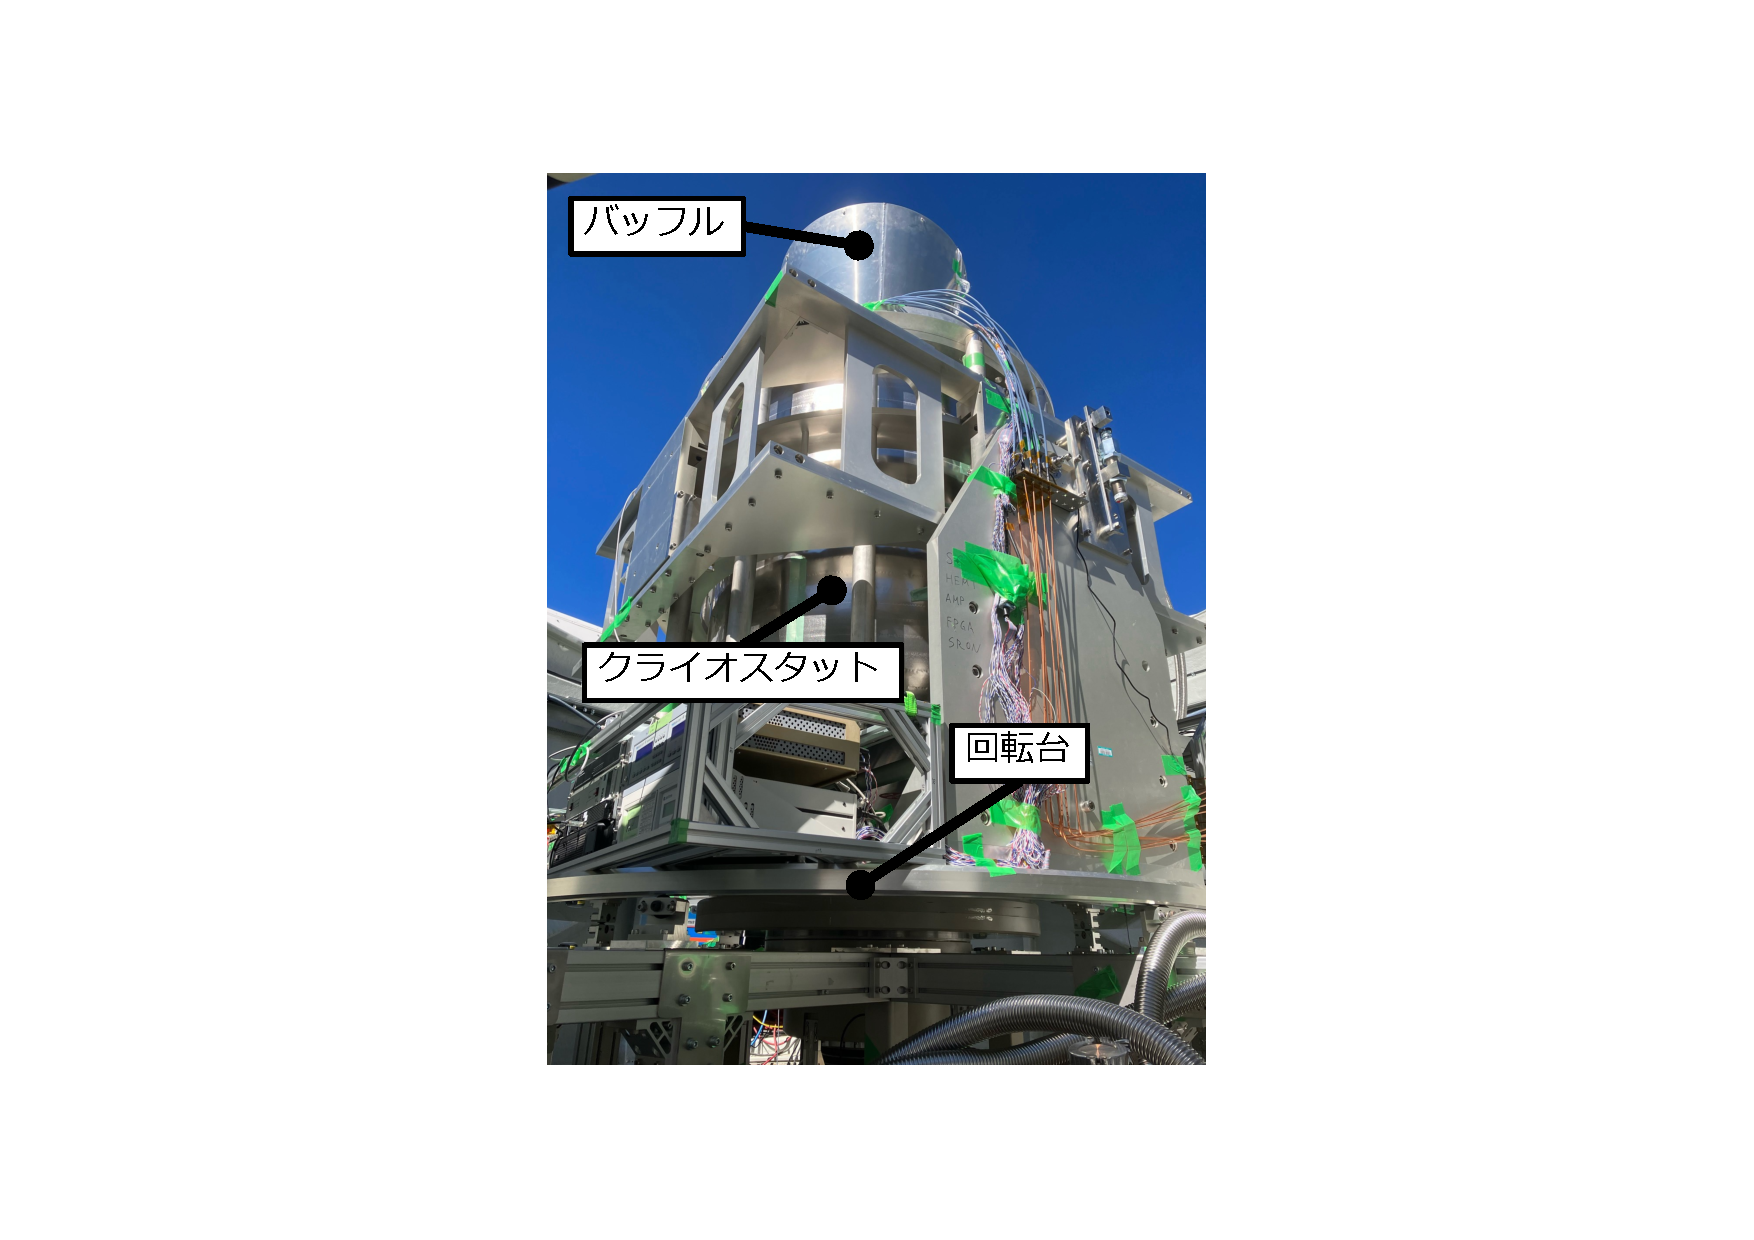
\includegraphics[width=0.5\columnwidth]{3_GB/figs/GB_overview2.pdf}
  \caption{GroundBIRD望遠鏡の外観。望遠鏡クライオスタットが方位角回転台の上に設置されており、回転台とともに最大で20RPM(1分間で20回転)の速度で回転する。}
  \label{GB_overview}
\end{figure}
\section{実験概要}

\subsection{GroundBIRD望遠鏡とスキャン戦略}
GroundBIRD望遠鏡はスペイン領カナリア諸島の1つであるテネリフェ島のテイデ観測所(高度2,400m)に位置する地上CMB望遠鏡である。地上からの観測において最も邪魔なのが大気からの放射であるが、テイデ観測所は大気中の積算水蒸気量(Precipitable Water Vapor、以下PWVと略す)がおよそ3.5mm\cite{PWV}と、観測に適した場所である。

\subsection{物理ターゲット}

\section{現在の観測状況}

\subsection{検出器のフルアレイインストール}

\subsection{リモート観測システム}
